%
%    F U K U D A
%


\documentclass[10pt,b5paper,papersize,dvipdfmx]{jsbook}
% 会誌は B5 サイズです

\usepackage{vuccaken}
\usepackage{vuccaken2019}

% スタイルファイルの読み込みや自作マクロは、
% 最終的には vuccaken2019.sty の中に書いてください。
% とりあえずはここに書いてもらって構いません。

% \newcommand\shiki[1]{\siki{#1}式}

\begin{document} % 以下本文

\mokuji{2} % 目次出力

% - - - - - - - - - - - - - - - - - - - - - - - - %
\kaishititle%
  {Re:マクスウェルから始める電磁気}% title
  {理工学部物理科学科1回生}% 所属
  {\vname{福田}{大和}}% name
% - - - - - - - - - - - - - - - - - - - - - - - - %

\section*{はじめに}
電磁気学の概要をかなーーーーーーーーーーーり駆け足で説明いたします。説明は私が学んだ中で最もしっくりきた本を基にしています。具体的には、多くの電磁気学の教科書はクーロンの法則などの、あまり電磁気学に触れたことのない方にも直感的に分かりやすい関係から初めて、マクスウェル方程式を導き、云々、という展開が一般的かと思います。しかし、今回は初めに電磁気学全てを支配するマクスウェル方程式を提示し、種々の関係を導くという順序です。間違っている可能性も十二分にあり得ますのでそのことに留意してお読みいただければ幸いです。

\section{注意事項}
\begin{itemize}
  \item ここではベクトルは太字で書きます。例えば、$A$というベクトルは$\vb*{A}$と書き、$\vec{A}$とは書きません。
  \item ベクトル解析の説明は一切ありません。
  \item 各語句については『マクスウェル方程式から始める電磁気学\cite{Maxwel}』に則るものとします。
\end{itemize}

\section{電磁気学概説}

\subsection{マクスウェル方程式}
まずは、電磁気学です。兎にも角にも、まずはマクスウェル方程式を見て頂きましょう。

\subsubsection{〈積分形〉}
\begin{numcases}
  {}
  \label{eq:Gauss}
  \int_S \vb*{E}\cdot \vb*{n} dS = \frac{1}{\epsilon_0} \int_V \rho dV \\
  \label{eq:Faraday}
  \oint_C \vb*{E}\cdot d\vb*{r} = -\frac{d}{dt}\int_S \vb*{B}\cdot\vb*{n} dS \\
  \label{eq:Gauss2}
  \int_S \vb*{B}\cdot \vb*{n} dS = 0 \\
  \label{eq:Ampere}
  c^2 \oint_C \vb*{B}\cdot d\vb*{r} = \frac{1}{\epsilon_0}\int_S \vb*{j}\cdot \vb*{n}dS + \frac{d}{dt}\int_S \vb*{E}\cdot \vb*{n} dS
\end{numcases}
以上の四つがマクスウェル方程式と呼ばれる、電磁気学全てを支配する方程式達です。
尚、文字の意味は$\vb*{E}$:電場、$\vb*{B}$:磁場、$\vb*{j}$:流束、$\vb*{n}$:法線ベクトル、$C$:任意の閉曲線、$S$:任意の閉曲面、$V$:任意の閉曲面Sに囲まれた体積、$\rho$:電荷密度です。\par
また、ここでは定数である光速$c$と真空の誘電率$\epsilon_0$を用いていますが、これらと真空の透磁率$\mu_0$の間には
\begin{align}
  c^2 \epsilon_0 \mu_0=1
\end{align}
の関係があるため、読む本によっては別の表記になっているかもしれません。
各方程式にはそれぞれ名前があり、\shiki{Gauss}はガウスの法則、\shiki{Faraday}はファラデーの法則、\shiki{Gauss2}は磁場に関するガウスの法則、\shiki{Ampere}はアンペール-マクスウェルの法則と呼ばれています。\shiki{Gauss}と\shiki{Faraday}が電場、\shiki{Gauss2}と\shiki{Ampere}が磁場に関する法則となんとなく考えて頂ければ結構です。

\subsubsection{〈微分形〉}
次に、積分形で書かれた上のマクスウェル方程式を微分形に変形したいと思います。 \par
まずはガウスの法則から。\shiki{Gauss}の左辺をガウスの定理で変形してやって、
\begin{align}
  \int_V \nabla\cdot\vb*{E} dV = \frac{1}{\epsilon_0} \int_V \rho dV
\end{align}
$V$は任意の体積としているので、
\begin{align}
  \nabla\cdot\vb*{E} = \frac{\rho}{\epsilon_0}
\end{align}
これがガウスの法則の微分形になります。\par
続いて、ファラデーの法則。\shiki{Faraday}の左辺にストークスの定理で変形してやって、
\begin{align}
  \int_S (\nabla\times\vb*{E})\cdot\vb*{n} dS = -\frac{d}{dt}\int_S \vb*{B}\cdot \vb*{n} dS
\end{align}
閉曲面$S$は時間変化しないとして、
\begin{align}
  \int_S (\nabla\times\vb*{E})\cdot\vb*{n} dS = -\int_S \frac{\partial\vb*{B}}{\partial t}\cdot \vb*{n} dS
\end{align}
$S$は任意の閉曲面としているので、
\begin{align}
  \nabla\times\vb*{E} = -\frac{\partial\vb*{B}}{\partial t}
\end{align}
これがファラデーの法則の微分形となります。
続いて、と行きたいところですが、磁場に関するガウスの法則とアンペール-マクスウェルの法則については、それぞれガウスの法則とファラデーの法則の変形と全く同じなので導出は割愛させていただきます\footnote{最後のおまけに一応掲載。}。結果だけ示すと、
\begin{align}
  \nabla\cdot \vb*{B} &= 0,\\
  c^2 \nabla\times\vb*{B} &= \frac{\vb*{j}}{\epsilon_o} + \frac{\partial\vb*{E}}{\partial t}
\end{align}
以上より、マクスウェル方程式の微分形をまとめると、
\begin{numcases}
  {}
  \label{eq:Gaussdif}
  \nabla\cdot\vb*{E} = \frac{\rho}{\epsilon_0}\\
  \label{eq:Faradaydif}
  \nabla\times\vb*{E} = -\frac{\partial\vb*{B}}{\partial t}\\
  \label{eq:Gauss2dif}
  \nabla\cdot \vb*{B} = 0\\
  \label{eq:Amperedif}
  c^2 \nabla\times\vb*{B} = \frac{\vb*{j}}{\epsilon_0} + \frac{\partial\vb*{E}}{\partial t}
\end{numcases}
となります。

\subsection{静電場}
さて、ここからは前章で提示したマクスウェル方程式をガチャガチャいじって楽しんでいこうと思います。まずは静電場。ここで使うのは以下の2式です。
\begin{numcases}
  {}
  \label{eq:Gauss1.2.2}
  \int_S \vb*{E}\cdot \vb*{n} dS = \frac{1}{\epsilon_0} \int_V \rho dV \\
  \label{eq:Faraday1.2.2}
  \oint_C \vb*{E}\cdot d\vb*{r} = 0
\end{numcases}
微分形だとこうなります。
\begin{numcases}
  {}
  \label{eq:Gaussdif1.2.2}
  \nabla\cdot\vb*{E} = \frac{\rho}{\epsilon_0}\\
  \label{eq:Faradaydif1.2.2}
  \nabla\times\vb*{E} = 0
\end{numcases}
はい、先程提示したガウスの法則とファラデーの法則です。が、少し違います。ファラデーの法則と\shiki{Faraday1.2.2}、\shiki{Faradaydif1.2.2}を見比べてみてください。右辺がどちらも$0$になっているのが分かるかと思います。これは静電場は時間変化しないから時間tで微分している項を$0$にしただけなのですが、この関係を{\bf 渦なしの法則}と呼びます。電場を閉曲線で線積分すると$0$になる、もしくは、電場の回転は$0$であると表現することもできます。これの何が重要なのか。それは保存力というものを考えると分かるかと思います。保存力という言葉は高校で既に聞き及んでいることと思いますが、改めて確認したいと思います。

\subsubsection{〈静電ポテンシャル〉}
力$\vb*{F}=(F_x,F_y,F_z)$を考えます。(電磁気学では普通、3次元の問題を取り扱うためこう置きましたが、何次元でも構いません\footnote{相対性理論を考慮すると3次元以外も考える必要があるようですが、勉強不足で分かりません! ……来年の今頃には分かるようになれるといいなぁ(遠い目)})この時、力$\vb*{F}$の成分が
\begin{align}
  \label{eq:consevativeP}
  F_x = -\frac{\partial U}{\partial x}, \quad
  F_y = -\frac{\partial U}{\partial y}, \quad
  F_z = -\frac{\partial U}{\partial z}
\end{align}
によって一つの関数$U(x,y,z)$から導かれるとき、この力は保存力である。\cite{mechanics}とのことです。\par
詳しく見ていきましょう。\shiki{consevativeP}を見てください。成分ごとに分けて書いているので分かりにくいかもしれないので、こう書いてみましょう。
\begin{align}
  \vb*{F}=\left(-\frac{\partial }{\partial x}U,-\frac{\partial }{\partial y}U , -\frac{\partial }{\partial z}U\right)
\end{align}
お分かりいただけましたか?つまり、
\begin{align}
  \label{eq:conservative}
  \vb*{F}=-\nabla U
\end{align}
こう書けます。この$U$を力学ではポテンシャル(位置エネルギー)と呼びます。\par
次に\shiki{conservative}の両辺を、任意の2点$A,B$の間を、任意の経路$r$で$A \to B$に線積分してみます。
% \begin{align}
% \int_A^B \vb*{F}\cdot d\vb*{r}=-\int_A^B \nabla U\cdot d\vb*{r}\\
% \label{eq:potential}
% \int_A^B \vb*{F}\cdot d\vb*{r}=U_A-U_B
% \end{align}
\begin{align}
  \int_A^B \vb*{F}\cdot d\vb*{r}
  = -\int_A^B \nabla U\cdot d\vb*{r}
  = U_A - U_B % 符号を反対にしました。あってます?
  \label{eq:potential}
\end{align}
\shiki{potential}は、保存力のする仕事は経路によらず、始点と終点のみで決まる、ということを表しています。ということは、当然、閉曲線で線積分すれば仕事は$0$になるのは自明です。\par
さて、保存力について認識したところで、改めてマクスウェル方程式を見てみましょう。
\begin{numcases}
  {}
  \int_S \vb*{E}\cdot \vb*{n} dS = \frac{1}{\epsilon_0} \int_V \rho dV \\
  \oint_C \vb*{E}\cdot d\vb*{r} = 0
\end{numcases}
\begin{numcases}
  {}
  \nabla\cdot\vb*{E} = \frac{\rho}{\epsilon_0}\\
  \nabla\times\vb*{E} = 0
\end{numcases}
電場$\vb*{E}$から働く力が保存力であるとわかると思います。つまり、渦なしの法則=電場は保存力、というわけです。そして、電場$\vb*{E}$は保存力なので、
\begin{align}
  \label{eq:Epotential}
  \vb*{E} = -\nabla\Phi
\end{align}
と書くことができ、$\Phi$を静電ポテンシャル(位置エネルギー)と呼びます。

\subsubsection{〈クーロンの法則〉}
次はクーロンの法則です。今回は積分形のマクスウェル方程式から求めていきます。\shiki{Gauss}と\shiki{Faraday}を使います。\shiki{Gauss}の$S$に半径$r$の球面(内側に点電荷$q$を持つ)をとると、\shiki{Gauss}は
\begin{align}
  \vb*{E}\cdot\vb*{n} \cdot 4\pi r^2 = \frac{\rho}{\epsilon_0}
\end{align}
右辺については、点電荷からの湧き出し全てを集めていると考えられるためこうなります。よって、
\begin{align}
  \vb*{E} = \frac{q}{4\pi\epsilon_0 r^2}\cdot\vb*{n}
\end{align}
これで一応クーロンの法則ではあるのですが、一般的な書き方とは異なるので書き直しておきます。
\begin{align}
  \vb*{E} = \frac{q}{4\pi\epsilon_0}\frac{\vb*{r}}{|r^3|}
\end{align}
または、点電荷の座標を$\vb*{r_0}$として、
\begin{align}
  \vb*{E} = \frac{q}{4\pi\epsilon_0}\frac{\vb*{r}-\vb*{r_0}}{|\vb*{r}-\vb*{r_0}|^3}
\end{align}
というように書くこともあります。どれも言っていることは同じです。

\subsubsection{〈ポアソン方程式〉}
次で静電場は最後になります。……最後に、してしまいます。\par
ここではポアソン方程式と呼ばれる関係式を紹介したいと思います。使うのは微分形の\shiki{Gaussdif1.2.2}です。まず、\shiki{Gaussdif1.2.2}の$\vb*{E}$に\shiki{Epotential}を代入すると、
\begin{align}
  \nabla\cdot(-\nabla\Phi ) =  \frac{\rho}{\epsilon_0}
\end{align}
これをラプラシアン$\nabla^2$を用いて書き直して、
\begin{align}
  \nabla^2 \Phi = - \frac{\rho}{\epsilon_0}
\end{align}
この式をポアソン方程式といいます。この式は微分方程式なので一般解が求められます。しかしここではポアソン方程式を直接解くことはせず、別の方法で一般解の一つを求めてみたいと思います。\par
クーロンの法則
\begin{align}
  \vb*{E} = \frac{q}{4\pi}\frac{\vb*{r}-\vb*{r}_0}{|\vb*{r}-\vb*{r}_0|^3}
\end{align}
から始めます。このクーロンの法則で表される電場について静電ポテンシャルを取ると
\begin{align}
  \Phi(\vb*{r}) = \frac{q}{4\pi\epsilon_0 r}-\frac{q}{4\pi\epsilon_0 r_0}
\end{align}
と書け、$r_0 = \infty$ととれば
\begin{align}
  \Phi(\vb*{r}) = \frac{q}{4\pi\epsilon_0 r}
\end{align}
ここで、$n$個の点電荷$q_1,q_2,\cdots,q_n$がそれぞれ$r_1,r_2,\cdots,r_n$にあるとすると、静電ポテンシャルは、
% \begin{align}
% \Phi(\vb*{r}) = \frac{1}{4\pi\epsilon_0}\sum_(i=1)^n \frac{q_i}{|\vb*{r}-\vb*{r_i}|} \\
% \Phi(\vb*{r}) = \frac{1}{4\pi\epsilon_0}\lim_(n \to \infty)\sum_(i=1)^n \frac{\rho(\vb*{r_i}) dV_i}{|\vb*{r}-\vb*{r_i}|}
% \end{align}
\begin{align}
  \Phi(\vb*{r}) 
  &= \frac{1}{4\pi\epsilon_0} \sum_{i=1}^n \frac{q_i}{|\vb*{r}-\vb*{r_i}|} \\
  &= \frac{1}{4\pi\epsilon_0}\lim_{n \to \infty} \sum_{i=1}^n \frac{\rho(\vb*{r_i}) dV_i}{|\vb*{r}-\vb*{r_i}|}
\end{align}
よって、体積分で表すと、
\begin{align}
  \Phi(\vb*{r}) = \frac{1}{4\pi\epsilon_0}\int_V \frac{\rho(\vb*{r}')}{|\vb*{r}-\vb*{r}'|}dV'
\end{align}
これがポアソン方程式の解の一つです。なぜこれがポアソン方程式の解といえるのかはクーロンの法則と重ね合わせの原理はポアソン方程式と静電ポテンシャルと同価であることに起因するのだが、今回は省略する。尚、注意点として、右辺の積分の変数は$\vb*{r}'$であることに注意してください。

\subsection{静磁場}
話は変わって、電場ではなく磁場について考えていきます。使うのは先程使わなかったマクスウェル方程式
\begin{numcases}
  {}
  \label{eq:Gauss2.1.2.3}
  \int_S \vb*{B}\cdot \vb*{n}dS = 0 \\
  \label{eq:Ampere1.2.3}
  c^2 \oint_C \vb*{B}\cdot d\vb*{r} = \frac{1}{\epsilon_0}\int_S \vb*{j}\cdot \vb*{n}dS
\end{numcases}
\shiki{Gauss2.1.2.3}と\shiki{Ampere1.2.3}です。微分形だとこうです。
\begin{numcases}
  {}
  \label{eq:Gauss2dif1.2.3}
  \nabla\cdot \vb*{B} = 0 \\
  \label{eq:Amperedif1.2.3}
  c^2 \nabla\times\vb*{B} = \frac{\vb*{j}}{\epsilon_0}
\end{numcases}
静磁場を考えるので、時間微分の項は全て消してあります。

\subsubsection{〈ベクトルポテンシャル〉}
最初に考えるのは、ベクトルポテンシャルというものです。\shiki{Gauss2dif1.2.3}をご覧ください。左辺に$\vb*{B}=\nabla\times\vb*{A}$というものを代入してみます。
% \begin{align}
% = \nabla\cdot(\nabla\times\vb*{A})
% \end{align}
\begin{align}
  \nabla\cdot \vb*{B} = \nabla\cdot(\nabla\times\vb*{A})
\end{align}
ベクトル解析における公式で、任意のベクトル$\vb*{r}$について、$\nabla\cdot(\nabla\vb*{r})=0$が成り立つので、
\begin{align}
  \nabla\cdot(\nabla\times\vb*{A})=0
\end{align}
が成立します。つまり、磁場$\vb*{B}$を$\nabla\times\vb*{A}$というもので置き換えても問題ないわけです。このベクトル$\vb*{A}$をベクトルポテンシャルといいます。\par
では、\shiki{Amperedif1.2.3}にも代入してみましょう。
\begin{align}
  c^2 \nabla\times(\nabla\times\vb*{A}) = \frac{\vb*{j}}{\epsilon_0}
\end{align}
これもベクトル解析の公式$\nabla\times(\nabla\times\vb*{A})=\nabla(\nabla\cdot\vb*{A})-\nabla^2\vb*{A}$を用いて、
\begin{align}
  \nabla(\nabla\cdot\vb*{A})-\nabla^2\vb*{A} = \frac{\vb*{j}}{\epsilon_0 c^2}
\end{align}
ここにクーロンゲージと呼ばれる制限$\nabla\cdot\vb*{A} = 0$を設けます。\par
これを用いて、
\begin{align}
  \nabla^2\vb*{A} = -\frac{\vb*{j}}{\epsilon_0 c^2}
\end{align}
ここから、この方程式を解いて、ベクトルポテンシャル$\vb*{A}$の解を求めなければならないのですが、お気づきでしょうか?この方程式、ポアソン方程式と全く同じ形をしています。つまり、ポアソン方程式の一般解を考えればよいのです。よって、
\begin{align}
  \label{eq:vecP}
  \vb*{A}(\vb*{r})
  = \frac{1}{4\pi\epsilon_0 c^2} \int_V \frac{\vb*{j}(\vb*{r}')}{|\vb*{r}-\vb*{r}'|} dV'
\end{align}
これがベクトルポテンシャルとなります。

\subsubsection{〈ビオ-サバールの法則〉}
続いて、先程求めたベクトルポテンシャルの式\shiki{vecP}を変形していきます。まず、両辺の回転をとると、
\begin{align}
  \vb*{B}(\vb*{r})
  = \nabla \left( \frac{1}{4\pi\epsilon_0 c^2} \int_V \frac{\vb*{j}(\vb*{r}')}{|\vb*{r}-\vb*{r}'|} dV' \right)
\end{align}
微分と積分の順序を入れ替えて、
\begin{align}
  \vb*{B}(\vb*{r})
  = \frac{1}{4\pi\epsilon_0 c^2} \int_V \nabla \times \frac{\vb*{j}(\vb*{r}')}{|\vb*{r}-\vb*{r}'|} dV'
\end{align}
この式の右辺を$\vb*{r}=(x,y,z)$の各成分で書き下すと、
\begin{numcases}
  {}
  \vb*{B}_x(\vb*{r})
    = \frac{1}{4\pi\epsilon_0 c^2} \int_V \frac{j_y(z-z') - j_z(y-y')}{|\vb*{r} - \vb*{r}'|^3}dV' \\
  \vb*{B}_y(\vb*{r})
    = \frac{1}{4\pi\epsilon_0 c^2} \int_V \frac{j_z(x-x') - j_x(z-z')}{|\vb*{r} - \vb*{r}'|^3}dV' \\
  \vb*{B}z(\vb*{r})
    = \frac{1}{4\pi\epsilon_0 c^2} \int_V \frac{j_x(y-y') - j_y(x-x')}{|\vb*{r} - \vb*{r}'|^3}dV'
\end{numcases}
よって、回転の定義を考えれば、
\begin{align}
  \vb*{B}(\vb*{r})
  = \frac{1}{4\pi\epsilon_0 c^2} \int_V \frac{\vb*{j}(\vb*{r}')\times(\vb*{r} - \vb*{r}')}{|\vb*{r} - \vb*{r}'|^3} dV'
\end{align}
これをビオ-サバールの法則といいます。

\subsection{時間変化}
電磁気学概説の最後は時間変化を考えていきます。使うのは当然、マクスウェル方程式4つ全てです。
\begin{numcases}
  {}
  \label{eq:Gauss1.2.4}
  \int_S \vb*{E}\cdot \vb*{n} dS
    = \frac{1}{\epsilon_0} \int_V \rho dV \\
  \label{eq:Faraday1.2.4}
  \oint_C \vb*{E}\cdot d\vb*{r}
    = -\frac{d}{dt} \int_S \vb*{B}\cdot\vb*{n} dS \\
  \label{eq:Gauss21.2.4}
  \int_S \vb*{B}\cdot \vb*{n} dS = 0 \\
  \label{eq:Ampere1.2.4}
  c^2 \oint_C \vb*{B}\cdot d\vb*{r}
    = \frac{1}{\epsilon_0} \int_S \vb*{j}\cdot \vb*{n}dS + \frac{d}{dt} \int_S \vb*{E}\cdot \vb*{n} dS
\end{numcases}
\begin{numcases}
  {}
  \label{eq:Gaussdif1.2.4}
  \nabla \cdot \vb*{E} = \frac{\rho}{\epsilon_0}\\
  \label{eq:Faradaydif1.2.4}
  \nabla \times \vb*{E} = -\frac{\partial\vb*{B}}{\partial t}\\
  \label{eq:Gauss2dif1.2.4}
  \nabla \cdot \vb*{B} = 0\\
  \label{eq:Amperedif1.2.4}
  c^2 \nabla \times \vb*{B}
    = \frac{\vb*{j}}{\epsilon_0} + \frac{\partial\vb*{E}}{\partial t}
\end{numcases}

\section{最後に}
あれ?時間変化は?と思うと思いますが、ページと時間(締切数時間前)と頭の関係上省略いたします。正直、後悔の残る出来なので、来年も電磁気の分野をテーマにリベンジしようと考えています。お読みいただきありがとうございます。おまけもあるので是非。

\section{おまけ}
\subsection{積分形→微分形}
\subsubsection{〈磁場に関するガウスの法則〉}
\begin{align}
  \int_S \vb*{B}\cdot \vb*{n}dS = 0
\end{align}
左辺にガウスの定理を適用して、
\begin{align}
  \int_V \nabla\cdot\vb*{B}dV = 0
\end{align}
$V$は任意の体積としているので、
\begin{align}
  \nabla\cdot\vb*{B} = 0
\end{align}

\subsubsection{〈アンペール-マクスウェルの法則〉}
\begin{align}
  c^2 \oint_C \vb*{B}\cdot d\vb*{r}
  = \frac{1}{\epsilon_0}\int_S \vb*{j}\cdot \vb*{n}dS + \frac{d}{dt}\int_S \vb*{E}\cdot \vb*{n}dS
\end{align}
左辺にストークスの定理を適用して、
\begin{align}
  c^2 \int_S (\nabla\times\vb*{B})\cdot\vb*{n}dS
  = \frac{1}{\epsilon_0}\int_S \vb*{j}\cdot \vb*{n}dS + \frac{d}{dt}\int_S \vb*{E}\cdot \vb*{n}dS
\end{align}
$S$は任意の閉曲面としているので、
\begin{align}
  c^2 \nabla\times\vb*{B} 
  = \frac{\vb*{j}}{\epsilon_0} + \frac{\partial\vb*{E}}{\partial t}
\end{align}

\subsection{微分形→積分形}
\subsubsection{〈ガウスの法則〉}
\begin{align}
  \nabla\cdot\vb*{E} = \frac{\rho}{\epsilon_0}
\end{align}
両辺を任意の体積$V$で積分して、
\begin{align}
  \int_V (\nabla\cdot\vb*{E})\cdot\vb*{n} dV = \int_V \frac{\rho}{\epsilon_0}dV
\end{align}
左辺にガウスの定理を適用して、
\begin{align}
  \int_S \vb*{E}\cdot \vb*{n} dS = \frac{1}{\epsilon_0} \int_V \rho dV
\end{align}

\subsubsection{〈ファラデーの法則〉}
\begin{align}
\nabla\times\vb*{E} = -\frac{\partial\vb*{B}}{\partial t}
\end{align}
両辺を閉曲面$S$で積分して、
\begin{align}
  \int_S (\nabla\times\vb*{E})\cdot\vb*{n} dS
  = -\int_S \frac{\partial\vb*{B}}{\partial t}\cdot\vb*{n} dS
\end{align}
左辺にストークスの定理を適用して、
\begin{align}
  \int_S (\nabla\times\vb*{E})\cdot\vb*{n} dS
  = -\frac{d}{dt} \int_S \vb*{B}\cdot\vb*{n} dS
\end{align}
他二つは省略。
\par

本編では何の前振りもなく使っていますが、一応ここでガウスの定理を証明しておきます。ストークスの定理も手順はほぼ同じなので省略します。

\subsubsection{〈ガウスの定理〉}
図\ref{fig:Gauss1}をご覧ください。
\begin{figure}[htbp]
  \centering
  % \begin{flushright}
  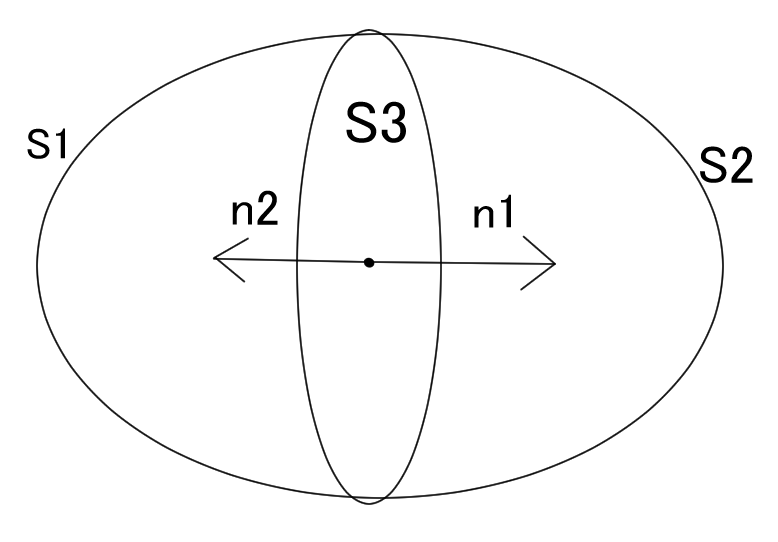
\includegraphics[width=5cm]{img/Gauss}
  \caption{}
  \label{fig:Gauss1}
  % \end{flushright}
\end{figure}
任意の閉曲面$S$を貫くベクトル場$\vb*{h}$の流束
\begin{align}
  \int_S \vb*{h}\cdot\vb*{n}dS
\end{align}
について考える。
$S = S_1 + S_2,\, S_a = S_1 + S_3,\, S_b = S_2 + S_3$として、
\begin{align}
  \int_{S_a} \vb*{h}\cdot\vb*{n}_1 dS + \int_{S_b} \vb*{h}\cdot\vb*{n}_2 dS 
  &= \int_{S_1} \vb*{h}\cdot\vb*{n} dS + \int_{S_3} \vb*{h}\cdot\vb*{n}_1dS \notag\\
  &\qquad + \int_{S_2} \vb*{h}\cdot\vb*{n}_2 dS + \int_{S_3} \vb*{h}\cdot\vb*{n}_2 dS 
\end{align}
$\vb*{n}_1 = \vb*{n}_2$のため、
\begin{align}
  \int_{S_a} \vb*{h}\cdot\vb*{n}_1 dS + \int_{S_b} \vb*{h}\cdot\vb*{n_2} dS
  &= \int_{S_1} \vb*{h}\cdot\vb*{n} dS + \int_{S_2} \vb*{h}\cdot\vb*{n}_2 \notag \\
  &= \int_S \vb*{h}\cdot\vb*{n} dS
\end{align}
よって、
\begin{align}
  \int_S \vb*{h}\cdot\vb*{n} dS
  = \lim_{N \to \infty} \sum_{i=1}^N \int_{S_i} \vb*{h}\cdot\vb*{n} dS
\end{align}
が得られる。

\begin{figure}[htbp]
  \centering
  % \begin{flushright}
  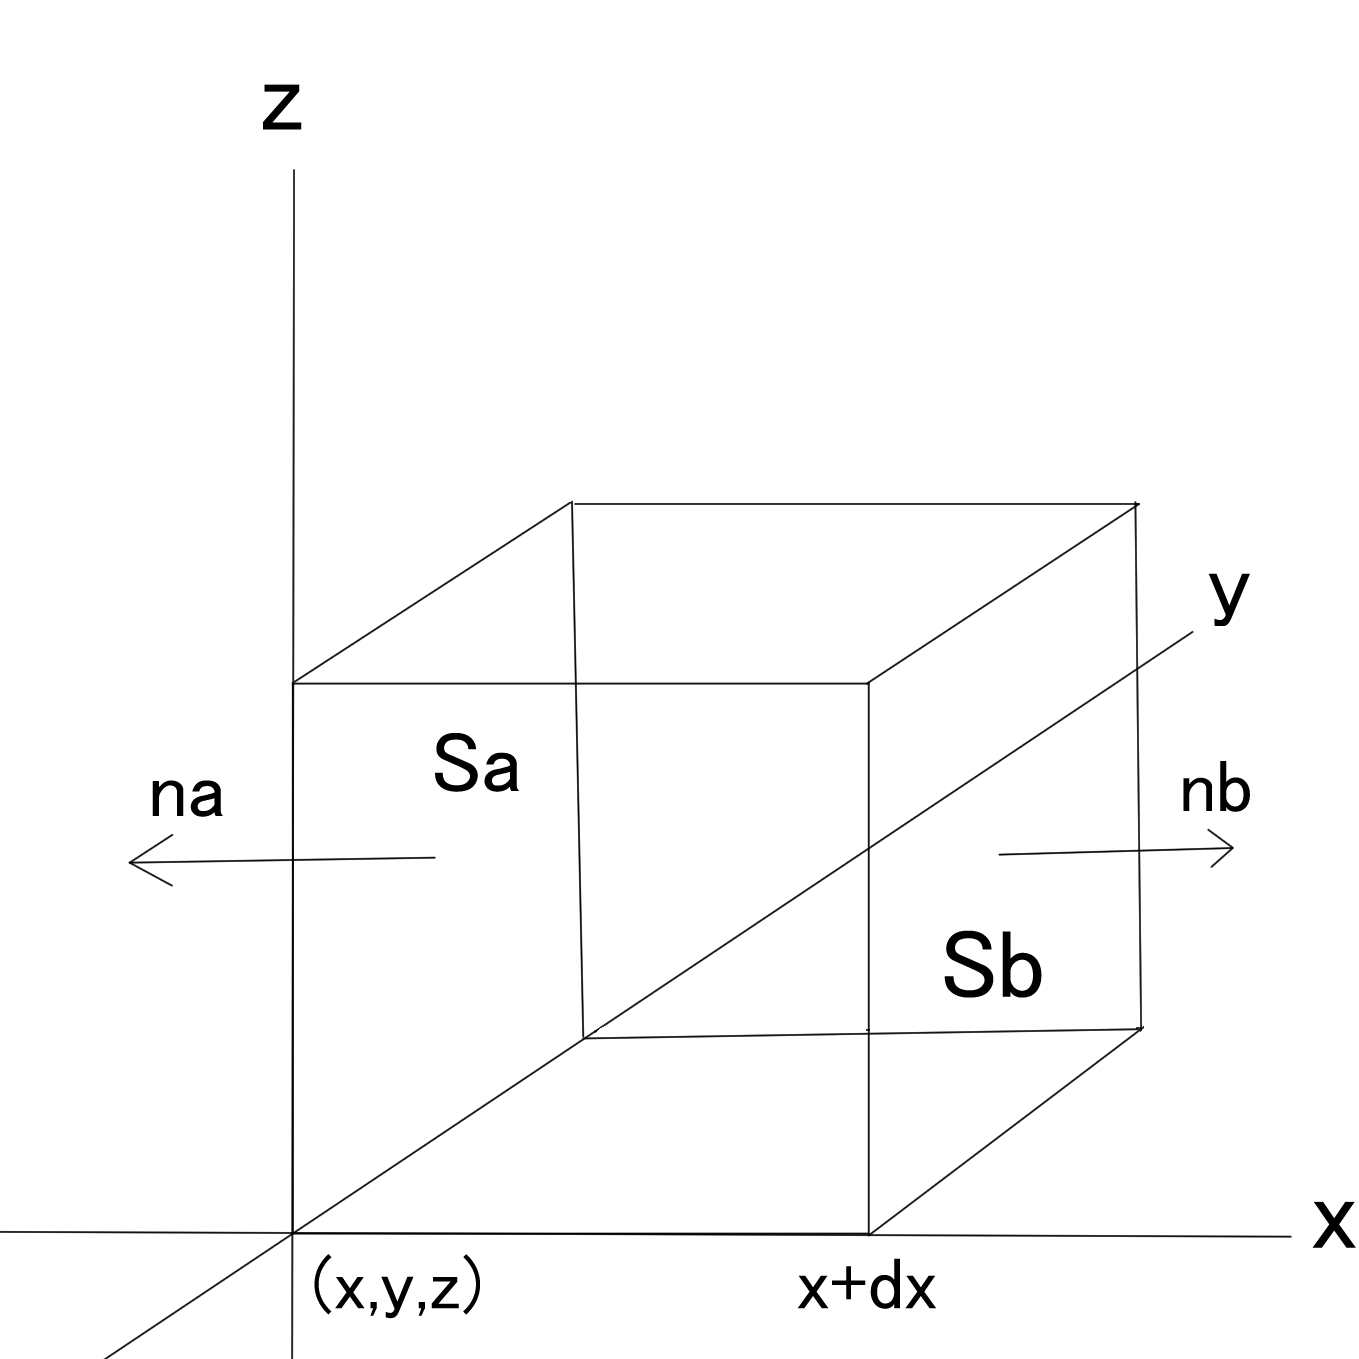
\includegraphics[width=5cm]{img/Gauss2}
  \caption{}
  \label{fig:Gauss2}
  % \end{flushright}
\end{figure}
次に図\ref{fig:Gauss2}についても流束を考えると、
\begin{align}
\int_{S_i} \vb*{h}\cdot\vb*{n}dS = \int_{S_a} \vb*{h}\cdot\vb*{n}_a dS + \int_{S_b} \vb*{h}\cdot\vb*{n}_b dS + \cdots
\end{align}
ここで$x$軸についてのみ流束を考えると、$\vb*{n}_a = \vb*{n}_b$より、
\begin{align}
  h_x = h_x(B) dydz
\end{align}
ただし、$\vb*{h} = (h_x,h_y,h_z),\, h_x(B)=h_x(x+dx,y,z)$である。ここで$h_x(B)$を偏微分を使って表して、
\begin{align}
  h_x(B)
  = h_x(x,y,z) + \frac{\partial h_x}{\partial x} dx
  = h_x(A) + \frac{\partial h_x}{\partial x} dx
\end{align}
よって、
\begin{align}
  \int_{S_a} \vb*{h}\cdot\vb*{n}_a dS + \int_{S_b} \vb*{h}\cdot\vb*{n}_b dS
  = \frac{\partial h_x}{\partial x} dxdydz
\end{align}
$y$軸、$z$軸についても同様に、
\begin{numcases}
  {}
  \frac{\partial h_y}{\partial y}dxdydz\\
  \frac{\partial h_z}{\partial z}dxdydz
\end{numcases}
よって、
\begin{align}
  \int_{S_i} \vb*{h}\cdot\vb*{n} dS = \nabla\cdot\vb*{h}dxdydz
\end{align}
$dxdydz$は$dV'$として、
\begin{align}
  \int_S \vb*{h}\cdot\vb*{n} dS = \lim_{N \to \infty} \sum_{i=1}^N \nabla\cdot\vb*{h} dV_i
\end{align}
つまり、
\begin{align}
  \int_S \vb*{h}\cdot\vb*{n} dS = \int_V \nabla\cdot\vb*{h} dV
\end{align}

%% 参考文献。thebibliography でいいです! nkymより
\begin{thebibliography}{9}
  % \bibitem{mechanics} 戸田 盛和,『物理入門コース 力学』,岩波書店,2017/12/5.
  \bibitem{mechanics} 戸田 盛和,『物理入門コース 力学』,岩波書店,2017.
  % \bibitem{Maxwel} 小宮山 進・竹川 敦,『マクスウェル方程式から始める電磁気学』,裳華房,2016/9/15 第二版.
  \bibitem{Maxwel} 小宮山 進・竹川 敦,『マクスウェル方程式から始める電磁気学』,裳華房,2016.
\end{thebibliography}

\end{document}


%\subsection{グラフや画像の挿入}
%\TeX はこれがめんどい。figure環境ごとコピペして使おう。
%
%\begin{figure}[htbp]
%  \centering
%  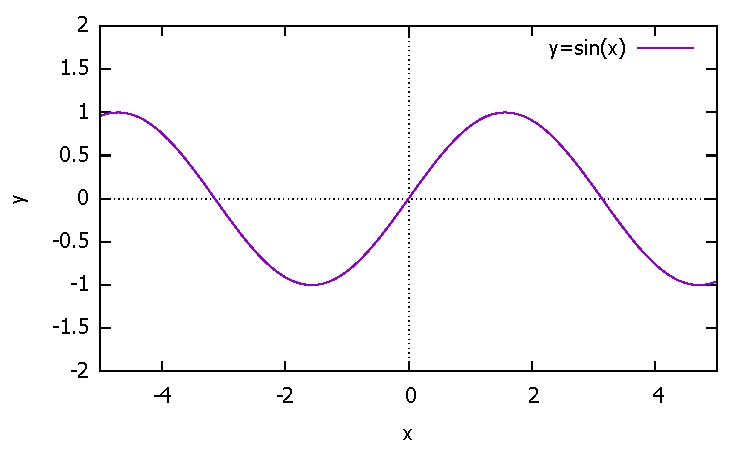
\includegraphics[width=10cm]{img/fig-sin.pdf}
%  \caption{$y=\sin x$のグラフ。gnuplotで作成した。}
%  \label{fig:sin}
%\end{figure}
%
%図\ref{fig:sin}より、sinが{\bfseries うねうね}であることがわかる。

%
%\subsection{ascmacパッケージ}
%枠で囲める。
%\begin{itembox}[l]{定義(ゼータ関数)}
%  $\Re(s) > 1$である任意の複素数$s$について、リーマンのゼータ関数$\zeta (s)$を以下のように定義する:
%  \begin{align*}
%    \zeta (s) := \sum_{n=1}^\infty \frac{1}{n^s}
%    \equiv \frac{1}{1^s} + \frac{1}{2^s} + \frac{1}{3^s} + \frac{1}{4^s} + \cdots
%  \end{align*}
%\end{itembox}

%
%\subsection{作図}
%\LaTeX と連携できるものとしては、picture環境やTi{\itshape k}ZやgnuplotやInkscapeなど色々な方法がありますが、ここではキーワードを挙げるに留めておきます。
%手描きを写真で撮ったり\footnote{明るさとコントラストをあげればそこそこキレイになる。}、パワポとかで作っても良いと思います\footnote{jpegは圧縮されて汚いので、pngか、ベクター形式のsvgとかpdfで作ると良い。}。

%
%\subsection{ソースコード}
%プログラムなどのソースコードを表示するにはlisting.styを使えばキレイに出力できますが、日本語に厳しい。そこで誰かが作ったplistings.styを代わりに使ってください。使い方はlisting.styと同じなので、そちらをキーワードにしてググってくだ
